\section{The CMSIS software library}
%
"The CMSIS is a set of tools, APIs, frameworks, and work flows that help to simplify software re-use, reduce the learning curve for microcontroller developers, speed-up project build and debug, and thus reduce the time to market for new applications. [...] CMSIS is open-source and collaboratively developed on GitHub : \url{https://github.com/ARM-software/CMSIS_5}." \\
\\
%
We will mostly be interested in the Digital Signal Processing (DSP) part of CMSIS, you can find the related documentation here: \url{https://arm-software.github.io/CMSIS_5/DSP/html/}. Be careful the version of this documentation does not match the one you find in your repo, you may notice some differences.\\
There are several \texttt{html} files that you can open with your browser. \\
From this link, you should find the doc on the data stuctures and functions in the column on the left side. For instance find information about the FFT function you will later use by clicking on \emph{Reference$\rightarrow$Transform functions$\rightarrow$Real FFT Functions$\rightarrow$arm \_rfft\_q15}.
%
\begin{figure}[H]
    \centering
    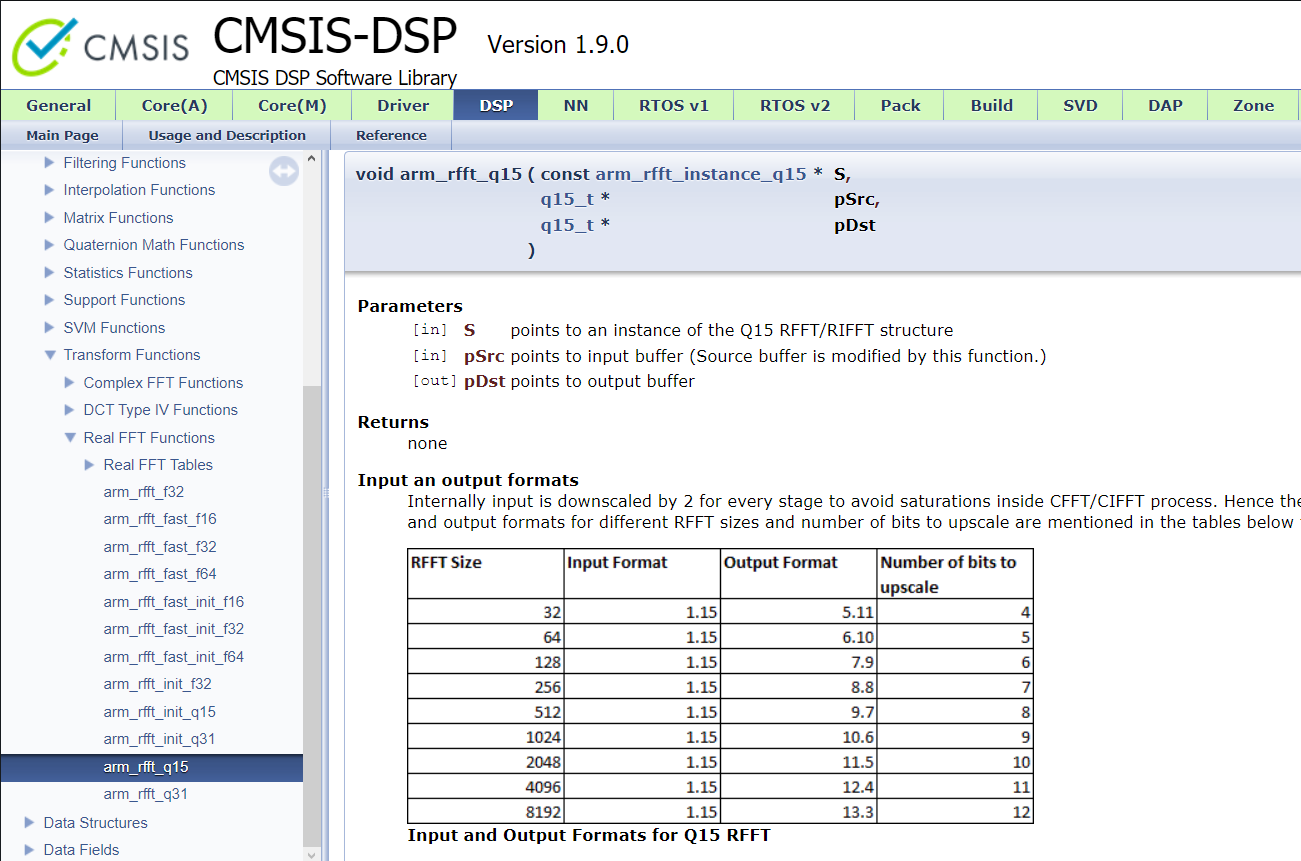
\includegraphics[width=\textwidth]{figs/CMSIS.png}
    \caption{CMSIS DSP doc.}
    \label{fig:CMSIS}
\end{figure}
%
\begin{bclogo}[couleur = gray!20, arrondi = 0.2, logo=\bcattention]{Don't trust CMSIS blindly}
Beware this documentation is far from exhaustive and often hides some subtleties, e.g. for \emph{arm\_rfft\_q15}:
%
\begin{itemize}
    \item The first coefficient of the output is real and equals $x[0]+x[N/2]$ for an input buffer $x$ of length $N$.
    \item The complex transforms used internally include scaling to prevent fixed-point overflows. The overall scaling equals 1/(fftLen/2). Due to the use of complex transform internally, the source buffer is modified by the rfft.
    \item Internally input is downscaled by 2 for every stage to avoid saturations inside CFFT process. Hence the output format is different for different RFFT sizes.
    \item If the input buffer is of length $N$, the output buffer must have length $2N$. The input buffer is modified by this function.
\end{itemize}
%
\begin{figure}[H]
\centering
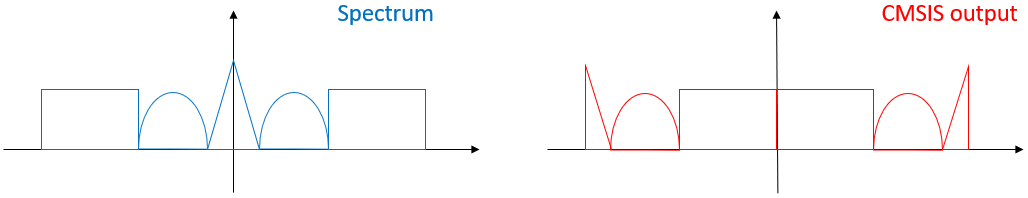
\includegraphics[width=\textwidth-4cm]{figs/CMSIS_output.PNG}
\caption{The FFT result starts with the DC component.}
\label{fig:CMSIS_output}
\end{figure}
\end{bclogo}
%
In a nutshell, making embedded computations in C-code using CMSIS-DSP is way more difficult than simple code with Python. This is why we provide you with a working implementation where we already took care you don't lose hours of debugging. \\
However, if you plan to change the way you compute your feature vector or anything else, you might probably take this time for it to work. \\
Note that these computations could also have been performed with floating point variables on your MCU (we started by this before jumping to fixed point).
